\documentclass[./main.tex]{subfiles}
\title{}
\begin{document}

\section{Quarter 2 Week 2-3 Update}

This past two weeks I created  a pipeline to start inference of admixture parameters on three different simple admixture models $\overrightarrow{(s_1,s_2,h)} = [(0.2,0.2,0.6),(0,0,1.0),(0.0001,0.2,0.7999)]$.  The plots below show the ancestry tract lengths of the different parameter sets aggregated for all chromosomes.


\begin{figure}[h]
     \centering
     \begin{subfigure}[b]{0.3\textwidth}
         \centering
    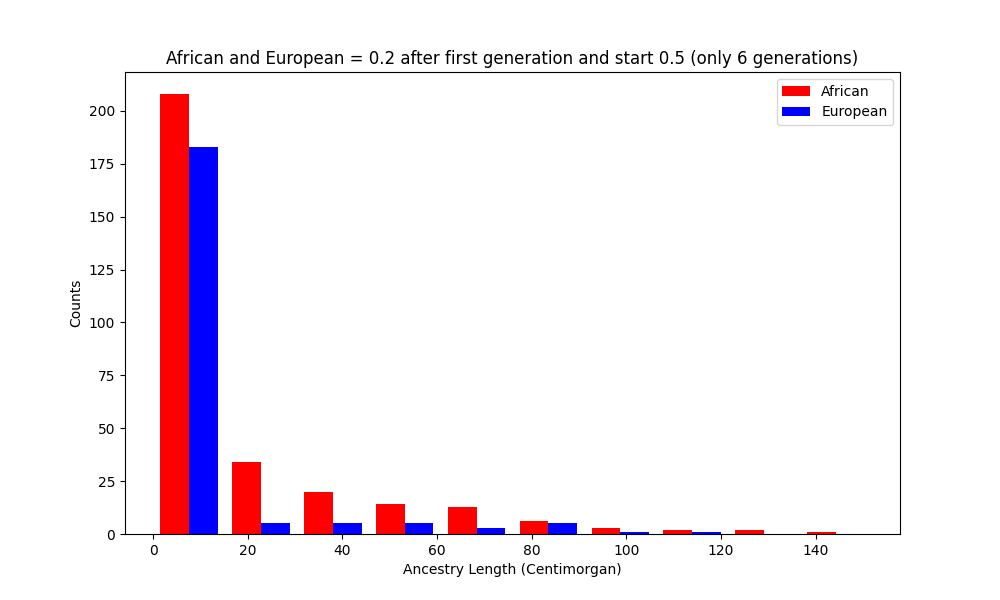
\includegraphics[width=1.0\linewidth]{Simulation_0_0.png}

    \label{fig:simple_1}
     \end{subfigure}
     \hfill
     \begin{subfigure}[b]{0.3\textwidth}
         \centering
    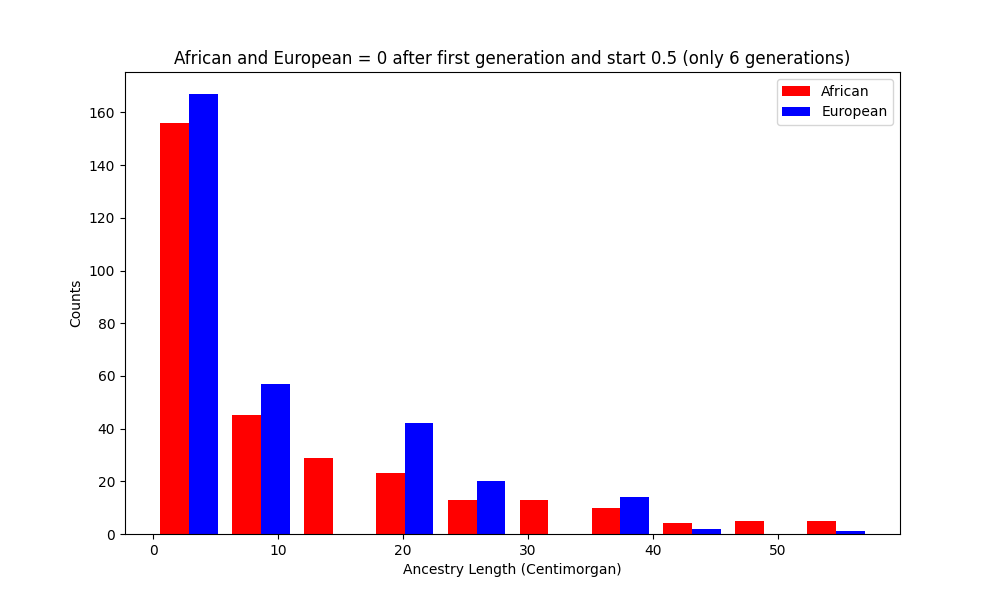
\includegraphics[width=1.0\linewidth]{Simulation_1_0.png}

    \label{fig:simple_1}
     \end{subfigure}
     \hfill
     \begin{subfigure}[b]{0.3\textwidth}
         \centering
    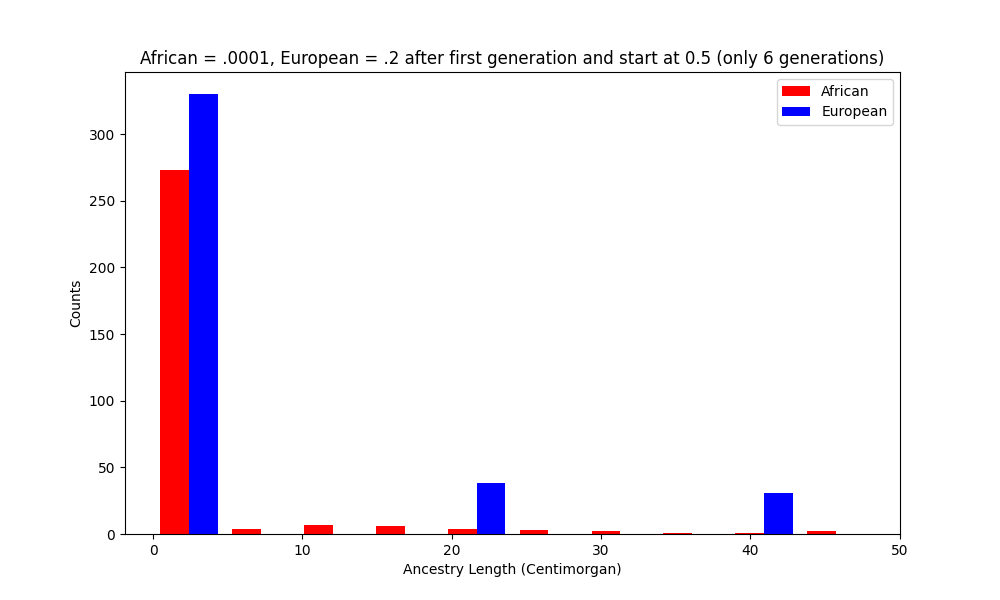
\includegraphics[width=1.0\linewidth]{Simulation_2_0.png}
    
    \label{fig:simple_1}
     \end{subfigure}
        \caption{Ancestry Tract Lengths with parameter set \\  $\overrightarrow{(s_1,s_2,h)} = [(0.2,0.2,0.6),(0,0,1.0),(0.0001,0.2,0.7999)]$}
        \label{fig:three graphs}
\end{figure}


\subsection{Admixture Parameters and thoughts}

Using a simple simulation based inference (ratio estimation) neural network architecture where the inputs are the ancestry tract lengths ($X$) and the simulation parameters ($\Theta$) we are able to achieve a mean squared error of 0.2 for simulations generated via constant parameters.  That means we are accurately learning the $P(X|(0.2,0.2,0.6)$ and the other parameter sets mentioned above.  This means we can use such a pipeline for inference of admixture parameters.

The more complicated scenario is having a new parameter set for every generation with a maximum of 15 generations, this means that each generation may have an admixture pulse or having an admixture pulse at specific generations.  This creates a more complicated scenario as we are trying to infer multiple parameters instead of just three distinct parameters (in the case of 2 founders).  Specifically this would require predicting an entire matrix rather than a vector.  

An idea to counter act this problem is to learn a lower representation of the matrix for the admixture parameters.  We can think of this as clustering, similar admixture parameter sets will be in the same cluster (and most likely generate similar ancestry tract lengths).  This could also allow us to create variable sized parameter sets i.e. less generations and we could just zero-pad the simulation parameters to the maximum generation time.  

Should we ignore pedigrees with only two parents ? 

What kind of architecture should we use for lower representation of parameter sets (transformers ??)

If the admixture fraction is very high, we run out of samples very quickly from the reference population set.  For example if $h=1.0$ we can only really go back 6 generations for European or African reference populations.  

\end{document}
